Our model was plagued by a number of small problems which we did not have the time to address. The most severe of these problems was our use of the incorrect equations \eqref{hLTD-wrong} and \eqref{Learning-wrong} presented in \cite{Fiete} instead of equations \eqref{hLTD} and \eqref{Learning}. Why are these equations wrong? In this model, hLTD depresses all synapses to or from a particular neuron if STDP alone would have pushed in synapses over the soft limit. However, the equations for \(\theta^{col},\theta^{row}\) check to see if \(W + \Delta^{STDP}\) increase beyond the soft limit. \(W + \Delta^{STDP}\) is a meaningless quantity. Instead, the equations should check to see if \(W + \eta\Delta^{STDP}\), which is equal to \(W\) updated by STDP alone, is greater than the soft limit. Equation \eqref{Learning-wrong} is not technically incorrect, since for different choices of \((\eta,\epsilon)\) it is equivalent to equation \eqref{Learning}. However, it introduces unnecessary complications, whereas equation \eqref{Learning} has two independent learning coefficients.

To see the effect of this, observe a graph of the error function starting from a permutation matrix with the correct method vs our implementation (figure \ref{EoT}):

\begin{figure}[H]
\centering
\begin{subfigure}[b]{0.49\textwidth}
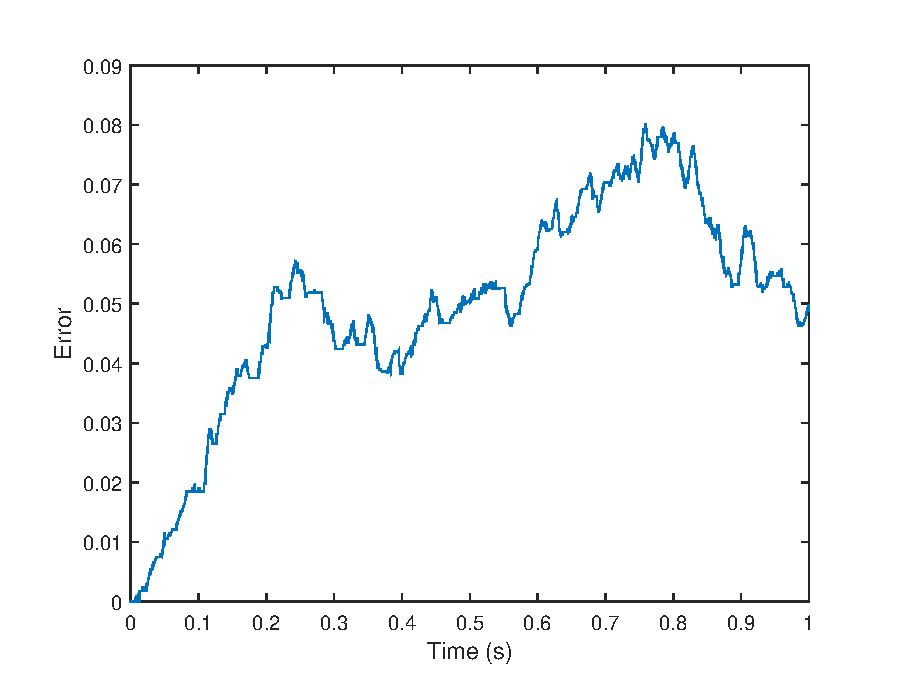
\includegraphics[width = \textwidth]{ErrorOverTime_6000Hz_perm_fixed.eps}
\caption{Error over Time, Corrected Method with \(r_{in} = 6000Hz\), \(\eta = 0.002\), \(\epsilon = 0.145\)}
\label{EoT: fixed}
\end{subfigure}
\,
\begin{subfigure}[b]{0.49\textwidth}
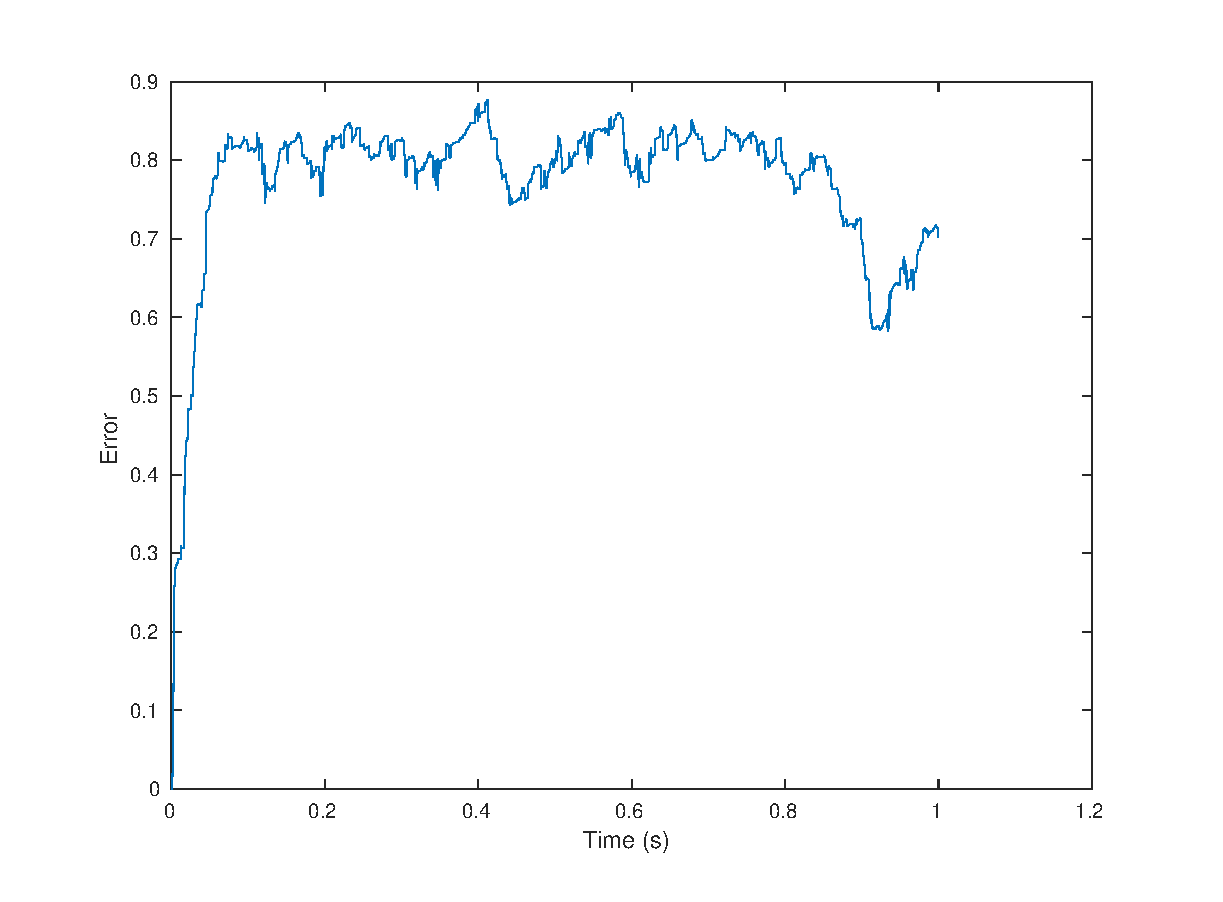
\includegraphics[width = \textwidth]{ErrorOverTime_6000Hz_Perm.eps}
\caption{Error over Time, Incorrect Method with \(r_{in} = 6000Hz\).}
\label{EoT: broken}
\end{subfigure}
\caption{It is clear that the error from the correct method is less than the error from the incorrect method by a factor of 10! This suggests most of the error seen earlier in the paper was due to a bad implementation, however even the corrected version has a certain constant error.}
\label{EoT}
\end{figure}

This implementation problem severely weakens our argument regarding the convergence of weight matrices under Hebbian plasticity. We were unable to amend this because the problem was caught too late for us to redo the simulations. 

However, even with the correct implementation, there seems to be a certain amount of structural error.

We also could have spent more time with parameter tuning. Most of our work on this project was spent trying to replicate the results of \cite{Fiete} using their model and parameters, but when the parameters didn't work as expected, we should have constructed our own. Ultimately, this did not prove a huge problem, because we were able to develop a working, stable IB neural network simulation.

The most interesting result of this paper is the hypothesis that learning methods other than STDP may be used to replicate the results of \cite{Fiete}. At the end of the results section, we provided a rough sketch of an argument that such learning rules combined with hLTD may cause the emergence of scaled permutation weight matrices. This argument could be formalized to categorize precisely which learning rules this would apply to.

Another interesting extension of this paper would be to generate permutation matrix behavior in a completely different network. For example, BCM's use of a moving threshold automatically triggers a heterosynaptic long-term depression event similar to that used in this model whenever the weighted total input to a neuron exceeds the threshold \cite{BCM}. BCM models are best applied to simple rate networks with output rates being linear or sigmoidal functions of the inputs. If such a network could be extended to a recurrent network and used to generate synfiring chains with weights converging to scaled permutation matrices, then this would provide further insight into how competition can be applied to learning to produce such firing patterns.